\documentclass[10pt,psamsfonts]{amsart}

%-------Packages---------
\usepackage{amssymb,amsfonts}
%\usepackage[all,arc]{xy}
\usepackage{enumerate}
%\usepackage{mathrsfs}
\usepackage{subcaption}
\usepackage{graphicx}
\usepackage{caption}
\usepackage{geometry}

%--------Theorem Environments--------
%theoremstyle{plain} --- default
\newtheorem{thm}{Theorem}[section]
\newtheorem{cor}[thm]{Corollary}
\newtheorem{prop}[thm]{Proposition}
\newtheorem{lem}[thm]{Lemma}
\newtheorem{conj}[thm]{Conjecture}
\newtheorem{quest}[thm]{Question}

\theoremstyle{definition}
\newtheorem{defn}[thm]{Definition}
\newtheorem{defns}[thm]{Definitions}
\newtheorem{con}[thm]{Construction}
\newtheorem{exmp}[thm]{Example}
\newtheorem{exmps}[thm]{Examples}
\newtheorem{notn}[thm]{Notation}
\newtheorem{notns}[thm]{Notations}
\newtheorem{addm}[thm]{Addendum}
\newtheorem{exer}[thm]{Exercise}

\theoremstyle{remark}
\newtheorem{rem}[thm]{Remark}
\newtheorem{rems}[thm]{Remarks}
\newtheorem{warn}[thm]{Warning}
\newtheorem{sch}[thm]{Scholium}

\makeatletter
\let\c@equation\c@thm
\makeatother
\numberwithin{equation}{section}

\bibliographystyle{plain}

%--------Meta Data: Fill in your info------
\title{Problem Set 3 \\ STAT 221}

\author{Won I. Lee}

%\date{July 30, 2016}


\begin{document}
	
\maketitle

\section*{1.1}

Please find the derivation below.

\begin{align*}
p(N,\theta) &= \int p(N,\theta|\lambda, \theta')p(\lambda, \theta')d\lambda d\theta'\\
&\propto \int \frac{(\lambda/\theta')^{-N}e^{-\lambda/\theta'}}{N!} \frac{1}{\lambda} 1_{\theta=\theta'}d\lambda d\theta\\
&\propto \frac{\theta^N}{N!}\int \frac{e^{-\lambda/\theta}}{\lambda^{N+1}}d\lambda\\
&= \frac{\theta^N}{N!} \int \frac{e^{-z}}{(\theta z)^{N+1}} \theta dz\\
&\propto \frac{1}{N!}\int e^{-z}/z^{N+1}dz\\
&\propto 1/N
\end{align*}
We find that after transformation, the prior on $N,\theta$ is precisely of the same form as $\lambda, \theta$. 

\section*{1.2}

No. To check, we simply integrate:
$$\int_0^1 \int_0^{\infty} \frac{1}{\lambda}d\lambda d\theta = \int_0^{\infty} \frac{1}{\lambda} d\lambda = \log \lambda |_{0}^{\infty}$$
which is not bounded.

\section*{1.3}

No. We first compute:
$$P(Y_i|\theta, \mu) = \sum_N P(Y_i|N, \theta) P(N|\theta, \mu) = \sum_N{N \choose Y_i} \theta^{Y_i}(1-\theta)^{N-Y_i} \frac{\mu^N e^{-\mu}}{N!}$$
$$ = \frac{e^{-\mu}\theta^{Y_i}}{Y_i!}\sum_N \frac{(1-\theta)^{N-Y_i}\mu^N}{(N-Y_i)!} = \frac{e^{-\mu\theta}(\mu\theta)^{Y_i}}{Y_i!}\sum_N \frac{[\mu(1-\theta)]^{N-Y_i}e^{-\mu(1-\theta)}}{(N-Y_i)!}$$
$$=\frac{e^{-\mu\theta}(\mu\theta)^{Y_i}}{Y_i!}$$
Thus, we have, letting $Y = Y_{1:n}$:
$$\log P(Y|\theta, \mu) = \sum_i \log P(Y_i|\theta, \mu) \propto \sum_i (Y_i\log \mu\theta - \mu\theta) = (\log\mu\theta) \sum_i Y_i - n\mu\theta$$
Taking derivatives, we find that:
$$\frac{\partial}{\partial \theta} \log P(Y|\mu, \theta) = \frac{n\bar{y}}{\theta} - n\mu$$
$$\frac{\partial}{\partial \mu} \log P(Y|\mu, \theta) = \frac{n\bar{y}}{\mu} - n\theta$$
Thus:
$$\frac{\partial^2}{\partial\theta^2}\log P(Y|\mu, \theta)  = -\frac{n\bar{y}}{\theta^2}$$
$$\frac{\partial^2}{\partial\theta\mu} \log P(Y|\mu, \theta)  = -n$$
$$\frac{\partial^2}{\partial \mu^2} \log P(Y|\mu, \theta)  = -\frac{n\bar{y}}{\mu^2}$$
The information matrix is then:
\begin{align*}
I(\theta,\mu) &= -E\left[ \frac{\partial^2}{\partial(\theta,\mu)^2} \log P(Y|\mu, \theta) |\theta,\mu \right]\\
&=n \begin{pmatrix} \mu/\theta & 1 \\ 1 & \theta/\mu \end{pmatrix}
\end{align*}
Now when we transform to $\theta, \lambda$ variables, we end up with an information matrix of the following form:
$$\tilde{I}(\theta, \lambda) = J^T I(\theta, \mu) J$$
where:
$$J = \left(\frac{\partial(\theta, \mu)}{\partial(\theta, \lambda)}\right)$$
But by the multiplication rule of determinants, we see that:
$$|\tilde{I}| = |J|^2 |I|$$
However, it is easy to see that $|I(\theta, \mu)| = 0$. Thus, we have that:
$$p(\lambda, \theta) \propto 1$$
or the uniform prior is non-informative in the sense of Jeffreys, and so the Raftery prior is not the Jeffreys' non-informative prior.

\section*{1.4}

We use a simple, symmetric proposal density for both $N, \theta$, namely:
$$N', \theta' | N, \theta \sim N + SBern(0.5) \cdot Pois(1), \mathcal{N}(\theta'|\theta, 0.05)$$
where $SBern$ is the symmetric Bernoulli distribution taking values $\pm 1$, and the two proposals are conditionally independent. We selected the parameters of the Poisson and Normal proposals based on experimentation and diagnostics of chain mixing for various parameter values. The results of our 10 chains for each dataset are given in {\bf Figure 1} and {\bf Figure 2}.

\begin{figure}
		\begin{subfigure}[b]{0.3\textwidth}
			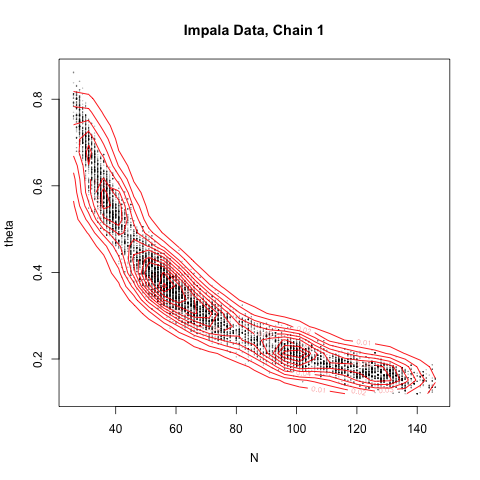
\includegraphics[width=\textwidth]{wonlee_mcmc_impala_1.png}
		\end{subfigure}
	\begin{subfigure}[b]{0.3\textwidth}
		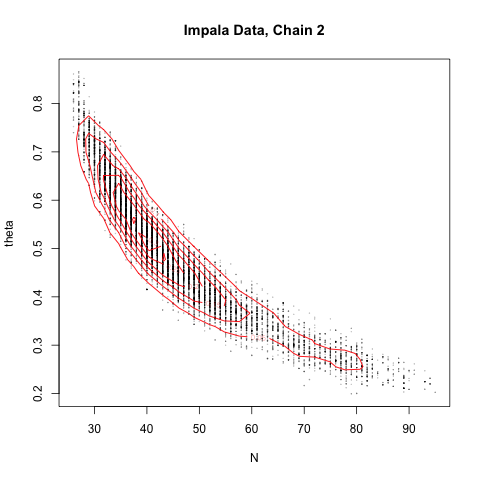
\includegraphics[width=\textwidth]{wonlee_mcmc_impala_2.png}
	\end{subfigure}
	\begin{subfigure}[b]{0.3\textwidth}
		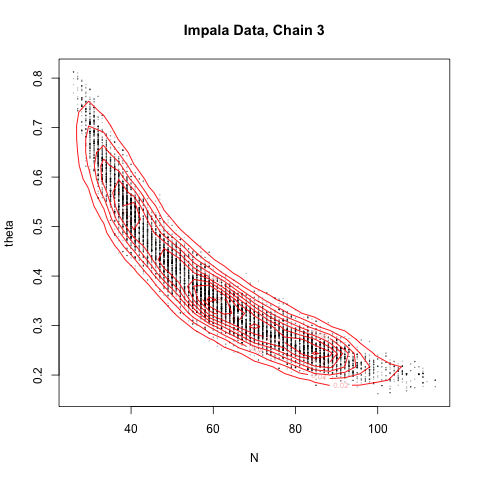
\includegraphics[width=\textwidth]{wonlee_mcmc_impala_3.png}
	\end{subfigure}
	\begin{subfigure}[b]{0.3\textwidth}
		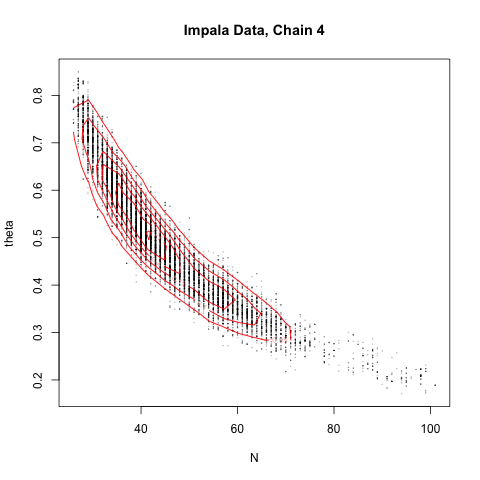
\includegraphics[width=\textwidth]{wonlee_mcmc_impala_4.png}
	\end{subfigure}
	\begin{subfigure}[b]{0.3\textwidth}
		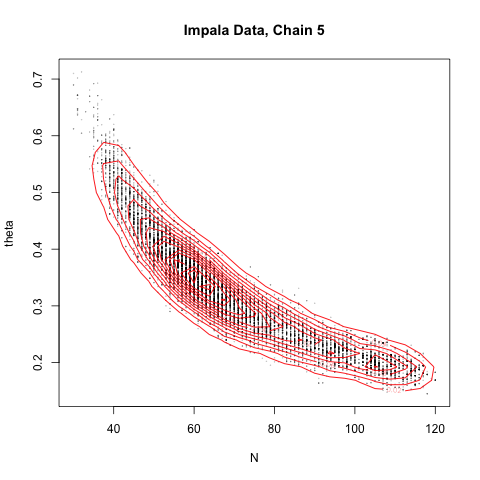
\includegraphics[width=\textwidth]{wonlee_mcmc_impala_5.png}
	\end{subfigure}
	\begin{subfigure}[b]{0.3\textwidth}
		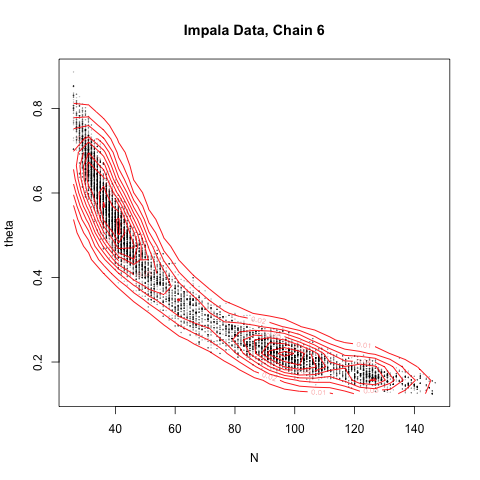
\includegraphics[width=\textwidth]{wonlee_mcmc_impala_6.png}
	\end{subfigure}
	\begin{subfigure}[b]{0.3\textwidth}
		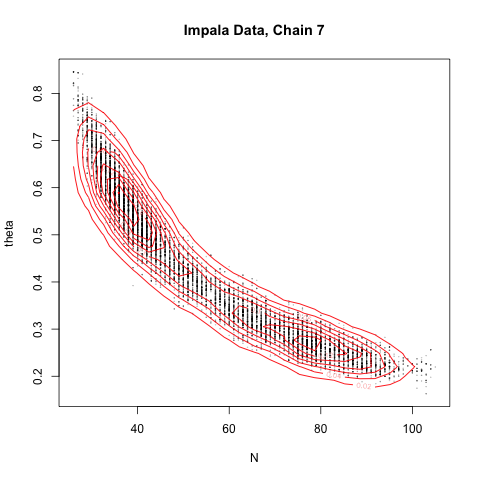
\includegraphics[width=\textwidth]{wonlee_mcmc_impala_7.png}
	\end{subfigure}
	\begin{subfigure}[b]{0.3\textwidth}
		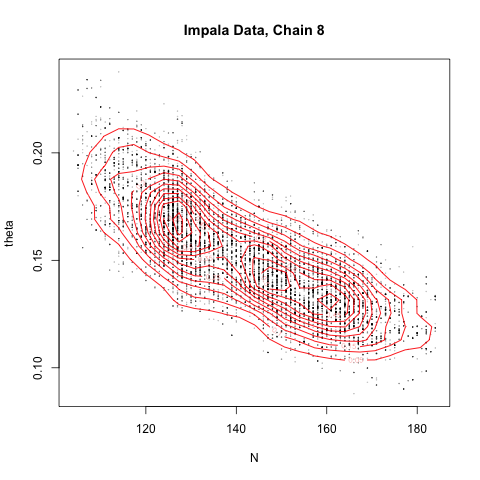
\includegraphics[width=\textwidth]{wonlee_mcmc_impala_8.png}
	\end{subfigure}
	\begin{subfigure}[b]{0.3\textwidth}
		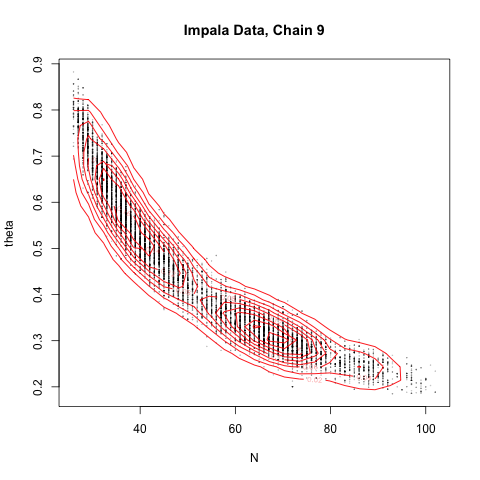
\includegraphics[width=\textwidth]{wonlee_mcmc_impala_9.png}
	\end{subfigure}
	\begin{subfigure}[b]{0.3\textwidth}
		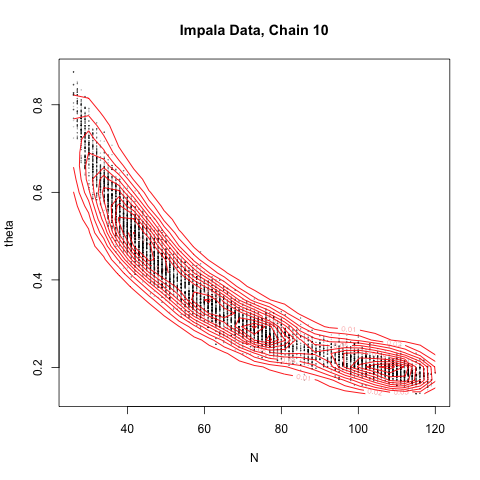
\includegraphics[width=\textwidth]{wonlee_mcmc_impala_10.png}
	\end{subfigure}
	\caption{MCMC posterior samples for Impala dataset}
\end{figure}

\begin{figure}
	\begin{subfigure}[b]{0.3\textwidth}
		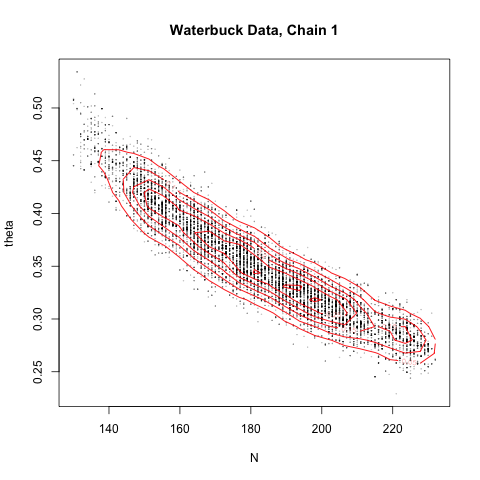
\includegraphics[width=\textwidth]{wonlee_mcmc_waterbuck_1.png}
	\end{subfigure}
	\begin{subfigure}[b]{0.3\textwidth}
		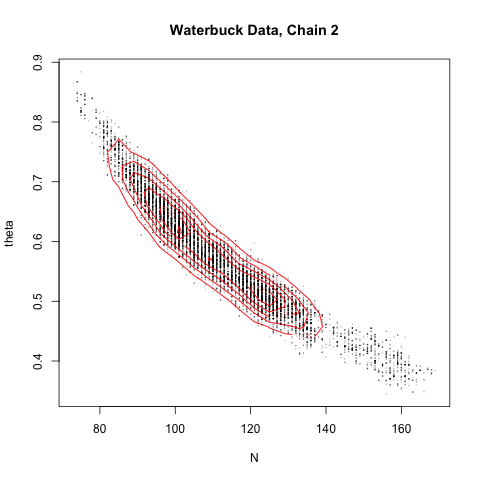
\includegraphics[width=\textwidth]{wonlee_mcmc_waterbuck_2.png}
	\end{subfigure}
	\begin{subfigure}[b]{0.3\textwidth}
		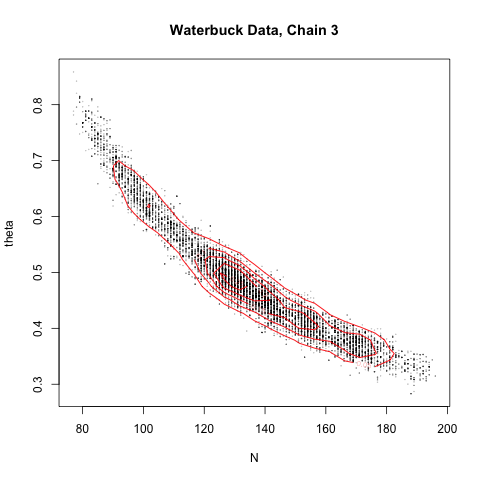
\includegraphics[width=\textwidth]{wonlee_mcmc_waterbuck_3.png}
	\end{subfigure}
	\begin{subfigure}[b]{0.3\textwidth}
		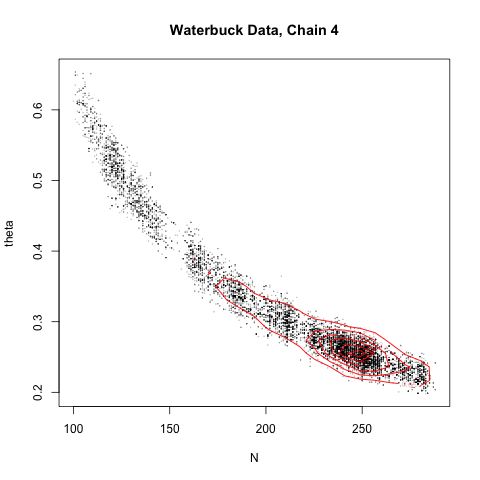
\includegraphics[width=\textwidth]{wonlee_mcmc_waterbuck_4.png}
	\end{subfigure}
	\begin{subfigure}[b]{0.3\textwidth}
		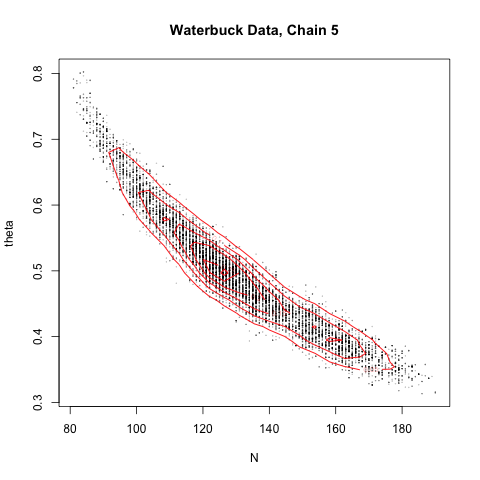
\includegraphics[width=\textwidth]{wonlee_mcmc_waterbuck_5.png}
	\end{subfigure}
	\begin{subfigure}[b]{0.3\textwidth}
		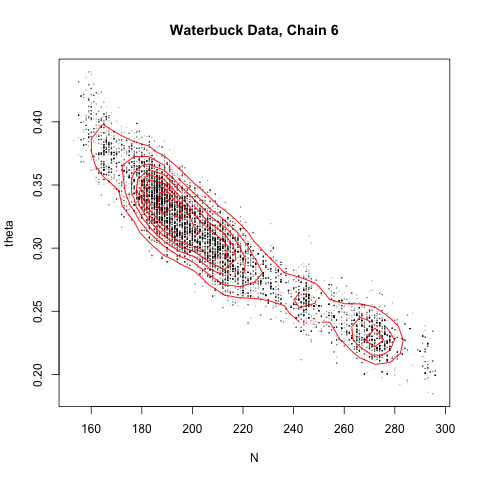
\includegraphics[width=\textwidth]{wonlee_mcmc_waterbuck_6.png}
	\end{subfigure}
	\begin{subfigure}[b]{0.3\textwidth}
		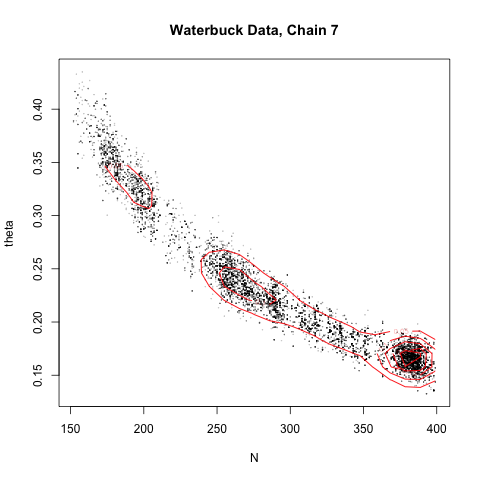
\includegraphics[width=\textwidth]{wonlee_mcmc_waterbuck_7.png}
	\end{subfigure}
	\begin{subfigure}[b]{0.3\textwidth}
		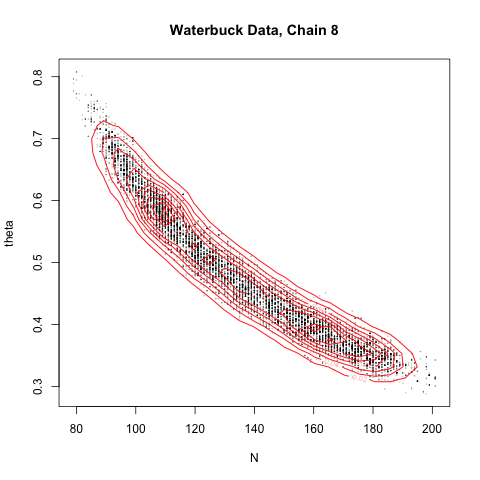
\includegraphics[width=\textwidth]{wonlee_mcmc_waterbuck_8.png}
	\end{subfigure}
	\begin{subfigure}[b]{0.3\textwidth}
		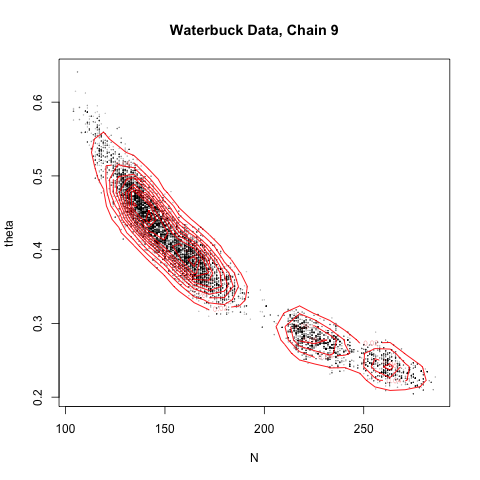
\includegraphics[width=\textwidth]{wonlee_mcmc_waterbuck_9.png}
	\end{subfigure}
	\begin{subfigure}[b]{0.3\textwidth}
		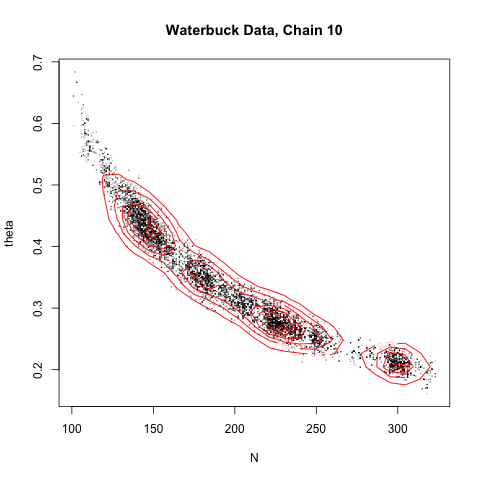
\includegraphics[width=\textwidth]{wonlee_mcmc_waterbuck_10.png}
	\end{subfigure}
	\caption{MCMC posterior samples for Waterbuck dataset}
\end{figure}

\section*{1.5}

We derive an unnormalized form of the marginal posterior as follows, again using shorthand where $Y = Y_{1:n}$.
\begin{align*}
P(N|Y) &\propto P(Y, N) = \int P(Y,N,\theta)d\theta\\
&= \int P(Y|N,\theta) P(N,\theta)d\theta\\
&\propto \frac{1}{N} \prod_{i=1}^n {N\choose y_i} \int \theta^{y_i} (1-\theta)^{N-y_i}d\theta\\
&= \frac{1}{N} \prod_{i=1}^n {N\choose y_i} \frac{\Gamma(n\bar{y}+1)\Gamma(n(N-\bar{y})+1)}{\Gamma(nN+2)}\\
&\propto\frac{(n\bar{y})!(n(N-\bar{y}))!}{N(nN+1)!} \prod_{i=1}^n {N\choose y_i}
\end{align*}
Note that while the $n\bar{y}$ term in the numerator is not strictly necessary since it does not depend on $N$, we leave it in the expression due to the fact that the numerical computations we conduct below yields numerical underflow without this term, even using Stirling's approximation.

We numerically sum these values for all reasonable values of $N$ to obtain the normalizing constant. Because the Waterbuck dataset presents challenges numerically for computing factorials and choose functions of large numbers, we employ Stirling's approximation beyond a certain $N > 250$ to compute the sum numerically. Thus:
$$Z = \sum_{N} P(N|Y) \approx \sum_{N=0}^{M} P(N|Y)$$
where $M$ is a large enough number; we employ $M = 2000$ to safely approximate the constant with enough probability mass. As shown in {\bf Figure 21}, we do indeed encompass most of the probability mass using this approximation.

\begin{figure}
	\centering
	\begin{subfigure}[b]{0.45\textwidth}
		\includegraphics[width=\textwidth]{wonlee_marginal_impala.png}
		\caption{Impala dataset}
	\end{subfigure}
	\begin{subfigure}[b]{0.45\textwidth}
		\includegraphics[width=\textwidth]{wonlee_marginal_waterbuck.png}
		\caption{Waterbuck dataset}
	\end{subfigure}
	\caption{Posterior marginal densities at various $N$ values for the Impala and Waterbuck datasets.}
\end{figure}

The normalizing constants we obtain are: $1.539\times 10^{-7}$ for Impala and $3.263\times 10^{-9}$ for Waterbuck.

\section*{1.6}

Using the numerically-normalized marginal $P(N|Y)$ above, we obtain:
$$P(N > 100|Y_{Impala}) \approx 0.3279$$
$$P(N > 100|Y_{Waterbuck}) \approx 0.9546$$
For our MCMC chains, we obtain posterior probabilities (averaging over the 10 chains) with standard deviations of:
$$\hat{P}(N>100|Y_{Impala}) \approx 0.169, \sigma \approx 0.305$$
$$\hat{P}(N>100|Y_{Waterbuck}) \approx 0.939, \sigma \approx 0.102$$
One immediate observation is that while the MCMC approximation for the Waterbuck dataset is reasonably close to the ``exact'' answer achieved by numerical integration, the MCMC approximation for the Impala dataset is far off the mark, yielding a posterior probability of around half the ``exact'' value.

This can be understood by again referring to {\bf Figure 21}. We note that while $N = 100$ is a reasonably high-probability value for the Waterbuck dataset, it is an extremely low-probability value for the Impala dataset. Consequently, it is likely that the MCMC sampler does not sufficiently explore this low-probability region of the posterior $N$ space during the sampling process, as the acceptance ratio is likely to be very low. On the other hand, the MCMC sampler likely has a reasonable probability of exploring the $N > 100$ region for the Waterbuck dataset since the posterior marginal is relatively high. This failure to explore in the Impala dataset can explain why the estimated probability is disastrously low for that dataset but reasonable close for the Waterbuck dataset. This intuition is confirmed by the standard deviation of the estimates, where the $\sigma$ for the Impala dataset probability estimate is much larger than that of the Waterbuck estimate, despite the estimated probability being lower.

\end{document}


